\documentclass{article}
\usepackage[paperletter]{geometry}
\geometry{top=1.0in, bottom=1.0in, left=1.0in, right=1.0in}
\usepackage[utf8]{inputenc}
\usepackage{cancel}
\usepackage{color, colortbl}
\definecolor{Gray}{gray}{0.9}
\usepackage{tikz}
\usepackage{siunitx}
\usepackage{amsmath}
\usepackage{mathdots}
\usepackage{yhmath}
\usepackage{color}
\usepackage{array}
\usepackage{multirow}
\usepackage{amssymb}
\usepackage{gensymb}
\usepackage{hyperref}
\hypersetup{
colorlinks=true,
linkcolor=blue,
filecolor=magenta,      
urlcolor=blue,
citecolor=blue,
}
\urlstyle{same}
\usepackage{tabularx}
\usepackage{booktabs}
\usepackage{booktabs}
\usepackage{float}
\usepackage{multicol}
\usetikzlibrary{fadings}
\usetikzlibrary{patterns}
\usetikzlibrary{shadows.blur}
\usepackage{fancyhdr}
\pagestyle{fancy}
\lfoot[\vspace{-15pt} \hline]{\vspace{-15pt} \hline}
\rfoot[\vspace{-15pt} \hline]{\vspace{-15pt} \hline}
\cfoot[\thepage]{\thepage}
\lhead[\copyright 2020 $-$ \textit{All Rights Reserved} ]{\copyright 2020 $-$ \textit{All Rights Reserved}}
\chead[AP Physics C]{AP Physics C}
\rhead[Michael Brodskiy]{Michael Brodskiy}
\usepackage[symbol]{footmisc}
\renewcommand*{\thefootnote}{\fnsymbol{footnote}}
%\usepackage{everysel}
%\usepackage{ragged2e}
%\renewcommand*\familydefault{\ttdefault}
%\EverySelectfont{%
%\fontdimen2\font=0.4em% interword space
%\fontdimen3\font=0.2em% interword stretch
%\fontdimen4\font=0.1em% interword shrink
%\fontdimen7\font=0.1em% extra space
%\hyphenchar\font=`\-% to allow hyphenation
%}
\title{Ice Puck Sliding Lab $-$ Acceleration at an Angle\\ AP \textsc{Physics} C}
\author{Michael \textsc{Brodskiy}}
\date{September 21, 2020}

\begin{document}

\maketitle
\begin{center}
\begin{tabular}{l r}
\underline{Date Performed}: & September 2020 \\\\ % Date the experiment was performed
\underline{Partners}: & Andrew Wang \\ & Yiying Zhang \\ & Salih Saygi \\\\
\underline{Instructor}: & Mrs. Morse \\\\\\\\\\ % Instructor/supervisor
\end{tabular}
\end{center}
\newpage

\tableofcontents
\listoftables
\listoffigures

\newpage
    
\section{Gathered Data}
\begin{center}
  
\begin{table}[H]\label{tab:Gathered Data} 
  \centering
\begin{tabular}{|l|l|}

  \hline
  Time $[\si{\second}]$ & Distance $[\si{\meter}]$ \\
  \hline
   0 & 0  \\
  \hline
  \rowcolor{Gray}
  .1 & .05  \\
  \hline
  .2 & .13 \\
  \hline
  \rowcolor{Gray}
  .3 & .26 \\
  \hline
  .4 & .44 \\
  \hline
  \rowcolor{Gray}
  .5 & .66 \\
  \hline
  .6 & .93 \\
  \hline
  \rowcolor{Gray}
  .7 & 1.24\\
  \hline
  .8 & 1.59\\
  \hline
\end{tabular}
\caption{Gathered Data}
\end{table}

\end{center}

\begin{enumerate}

  \item Mass = $.42[\si{\kilo\gram}]$

\item Angle = $28\degree$

\end{enumerate}

\end{enumerate}

\section{Statement of Purpose}

\begin{justify} This laboratory experiment is intended to calculate the acceleration at a predetermined angle ($28\degree$ in this case).  \end{justify}

\section{Materials Used}

\begin{enumerate}

  \item Ice Puck

  \item Timer

  \item Inclined Slope

  \item Ruler

  \item Protractor

  \item Pivot Interactives Lab

\end{enumerate}
\newpage

\section{Procedure}

\begin{justify}

  An ice puck of mass $m$ is placed on a slope inclined at $\alpha=28\degree$, measured from the tabletop to the lower side of the ramp. The ice puck is attached to a rope and at rest, until the rope is cut. The ice puck travels a total distance of $\Delta d =1.59[\si{\meter}]$. The distance traveled by the ice puck at each time $t=.1[\si{\second}]$ subinterval is measured. Friction is negligible. A diagram is shown below \ref{fig:diag}.

\end{justify}

\begin{figure}[H]
  \centering
  

\tikzset{every picture/.style={line width=0.75pt}} %set default line width to 0.75pt        

\begin{tikzpicture}[x=0.75pt,y=0.75pt,yscale=-1,xscale=1]
%uncomment if require: \path (0,461); %set diagram left start at 0, and has height of 461

%Shape: Can [id:dp17510382575383798] 
\draw   (359,350.95) -- (359,360.05) .. controls (359,361.13) and (345.57,362) .. (329,362) .. controls (312.43,362) and (299,361.13) .. (299,360.05) -- (299,350.95) .. controls (299,349.87) and (312.43,349) .. (329,349) .. controls (345.57,349) and (359,349.87) .. (359,350.95) .. controls (359,352.03) and (345.57,352.9) .. (329,352.9) .. controls (312.43,352.9) and (299,352.03) .. (299,350.95) ;
%Straight Lines [id:da6852491752642553] 
\draw    (151.5,363) -- (329,362) ;
%Shape: Boxed Line [id:dp20101918104290828] 
\draw    (329,362) -- (506.5,361) ;
%Shape: Arc [id:dp936530189477714] 
\draw  [draw opacity=0] (151.5,363.16) .. controls (151.5,362.51) and (151.5,361.86) .. (151.5,361.21) .. controls (151.5,235.71) and (230.97,133.97) .. (329,133.97) .. controls (426.97,133.97) and (506.41,235.59) .. (506.5,360.99) -- (329,361.21) -- cycle ; \draw   (151.5,363.16) .. controls (151.5,362.51) and (151.5,361.86) .. (151.5,361.21) .. controls (151.5,235.71) and (230.97,133.97) .. (329,133.97) .. controls (426.97,133.97) and (506.41,235.59) .. (506.5,360.99) ;
%Curve Lines [id:da6906058744459618] 
\draw    (304.5,136) .. controls (344.5,106) and (272.5,100) .. (312.5,70) ;
%Curve Lines [id:da5971348186954979] 
\draw    (357.5,137) .. controls (397.5,107) and (325.5,101) .. (365.5,71) ;

%Curve Lines [id:da43819511514532783] 
\draw    (310.5,71) .. controls (350.5,41) and (278.5,35) .. (318.5,5) ;
%Curve Lines [id:da3524822593890953] 
\draw    (363.5,72) .. controls (403.5,42) and (331.5,36) .. (371.5,6) ;

%Shape: Arc [id:dp13203389786079556] 
\draw  [draw opacity=0] (299,350.95) .. controls (289.62,342.24) and (283.69,329.37) .. (283.69,315.01) .. controls (283.69,288.78) and (303.5,267.51) .. (327.94,267.51) .. controls (352.37,267.51) and (372.19,288.78) .. (372.19,315.01) .. controls (372.19,328.96) and (366.59,341.5) .. (357.67,350.19) -- (327.94,315.01) -- cycle ; \draw   (299,350.95) .. controls (289.62,342.24) and (283.69,329.37) .. (283.69,315.01) .. controls (283.69,288.78) and (303.5,267.51) .. (327.94,267.51) .. controls (352.37,267.51) and (372.19,288.78) .. (372.19,315.01) .. controls (372.19,328.96) and (366.59,341.5) .. (357.67,350.19) ;
%Straight Lines [id:da08347245437858009] 
\draw    (291.5,315) -- (361.5,315) ;
%Straight Lines [id:da9255606880484] 
\draw    (291.5,298.25) -- (291.5,331.75) ;
%Straight Lines [id:da9160639670883368] 
\draw    (361.5,298.25) -- (361.5,331.75) ;

% Text Node
\draw (327.94,312.01) node [anchor=south] [inner sep=0.75pt]   [align=left] {$\displaystyle d$};


\end{tikzpicture}

  \caption{Setup of the Laboratory Experiment}
  \label{fig:diag}
\end{figure}

\section{Background Knowledge}

\begin{justify}

  For this laboratory experiment, it is necessary to know the three equations for uniformly accelerated motion \eqref{eq1}:

\end{justify}

\begin{equation}
  \begin{split}
    v_f=v_o+at \\
    \Delta x=v_ot+\frac{1}{2}at^2 \\
    v_f^2=v_o^2+2a\Delta x
  \end{split}
  \label{eq1}
\end{equation}

\section{Graphical Analysis}

\begin{figure}[H]
  \centering
  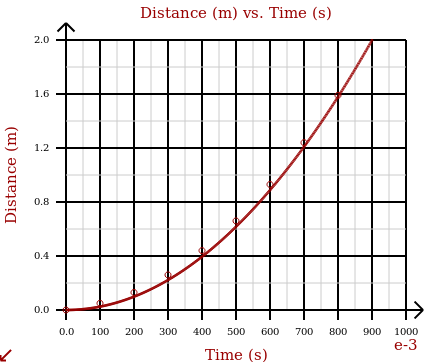
\includegraphics[width=.7\textwidth]{Figures/Curved.png}
  \caption{Non-linearized Data}
  \label{fig:curve}
\end{figure}

\begin{figure}[H]
  \centering
  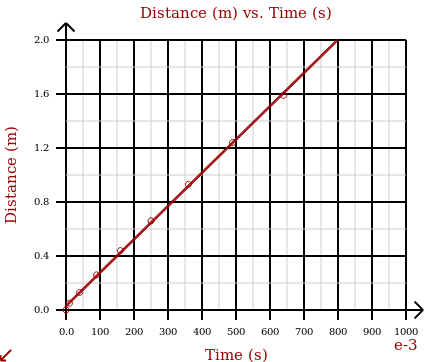
\includegraphics[width=.7\textwidth]{Figures/Linear.png}
  \caption{Linearized Data, $d=2.467t^2+.02978$}
  \label{fig:linear}
\end{figure}

  $$\text{The equation yielded by the linearized graph (\ref{fig:linear})  is: } d=2.467t^2+.02978 \text{ or } d=2.467s+.02978, $$
$$\text{where variables substitution } (s = t^2) \text{ is used to keep the function in linear terms.}$$
$$\text{Thus, the slope is } 2.467\left[\frac{\si{\meter}}{\si{\second\squared}}\right], \text{ as this value represents the acceleration of the ice puck.}$$

\section{Mathematical Analysis}

\begin{justify}

  First of all, it is necessary to solve for the acceleration attained using our data, by plugging the slope into the second kinematics equation found in equation list one \eqref{eq1}. This is done in equation two \eqref{eq2}:

\end{justify}

\begin{equation}
  \begin{split}
    \frac{1}{2}a & = 2.467\\
    a & = 2\cdot 2.467 \\
    & = 4.934\left[ \frac{\si{\meter}}{\si{\second\squared}} \right]
  \end{split}
  \label{eq2}
\end{equation}

\begin{justify}

Next, it is necessary to solve for the theoretical acceleration, determined by $a=g\sin(\theta)$. The theoretical acceleration is found in equation three \eqref{eq:3}:

\end{justify}

\begin{equation}
  \begin{split}
    g & = 9.80665\left[ \frac{\si{\meter}}{\si{\second\squared}} \right]\\
    a & = g\sin(28\degree) \\
    & = 4.9033\left[ \frac{\si{\meter}}{\si{\second\squared}} \right]
  \end{split}
  \label{eq:3}
\end{equation}

\begin{justify}

  Finally, the percent error must be calculated by the formula provided in equation 4 (where $t$ is the theoretical value and $x$ is the experimental value) \eqref{eq:4}. The calculation for the percent of error is provided in equation 5 \eqref{eq:5}:

\end{justify}

\begin{equation}
  \%_{error}=\frac{|x-t|}{t}\cdot 100\%
  \label{eq:4}
\end{equation}

\begin{equation}
  \begin{split}
    \%_{error} & = \frac{|4.934-4.9033|}{4.9033}\cdot 100\% \\
    & = .626\%
  \end{split}
  \label{eq:5}
\end{equation}

\section{Conclusion and Analysis}

\begin{justify}

  Following the experimentation, it is evident that, as the angle approaches $90\degree$, the acceleration approaches $g$. This can be concluded analytically, as the formula for the theoretical acceleration is $a=g\sin(\theta)$. Therefore, as the angle approaches $90\degree$, $\sin(\theta)$ approaches one, and, overall, $a$ approaches $g\cdot1$, or $g$. A calculation for percent error is performed in \eqref{eq:5}. Our margin of error was $.626\%$, which means that the value provided from the linearization of our data was very accurate. It is difficult to name sources of error, as this lab was performed virtually; however, a few come to mind. First of all, the force of friction should not actually be negligible. This should mean that our value for acceleration is less than the theoretical value, however, this is proven untrue in our scenario. Another possible source of error is the damage done to the puck after use. With every use, the surface of the puck becomes more rough, which converts to a greater friction, which, in turn, means less acceleration. These possible sources of error, though, are quite trivial, and, therefore, do not have a significant effect of the data. As our collected data shows, the correlation between our experimental acceleration and the theoretical acceleration is very close. An interesting future experiment would be something similar to this, but involving the force of friction $-$ something like ``the effects of mass on the force of friction.''

\end{justify}

\end{document}
